\section{Approach} 
\label{approach}

\subsection{Overview} 
\label{ch:approach0}

The epistemic research interest in this work is to clarify the question, whether conventional machine learning methods combined with suitable features can outperform neural network based approaches.

\begin{figure}[ht]
	\centering
	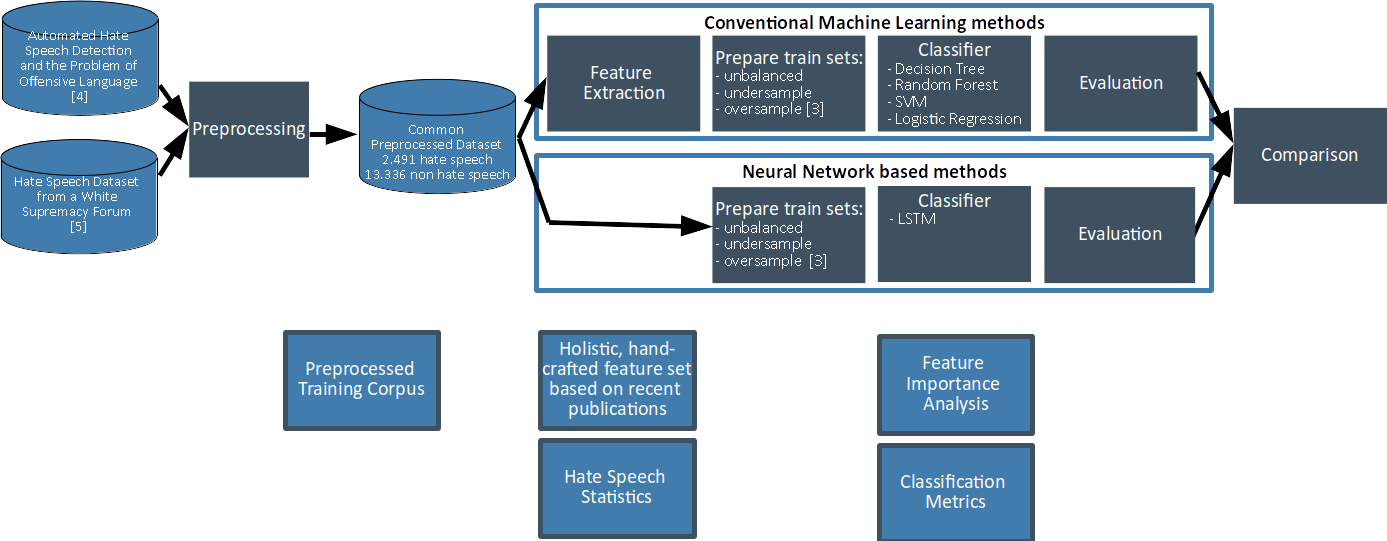
\includegraphics[width=1.0\linewidth]{figures/pipeline.png}
	\caption{Approach}
	\label{fig:overall_pipeline}
\end{figure}

Figure \ref{fig:overall_pipeline} visualizes our approach (on the top) and the resulting novelties achieved through this work (at the bottom). The following chapters describe the different steps in detail. First the data is merged and preprocessed resulting in a preprocessed training corpus. The next step differs between conventional machine learning methods and neural network based approaches. For conventional machine learning methods an explicit feature extraction is necessary. Therefore achievements of recent publications were combined to build a holistic, hand-crafted feature set. Based on these features, hate speech statistics could be further analyzed. Due to the fact that the common preprocessed corpus is unbalanced, an unbalanced, oversampled and under\-sampled dataset was created for further investigation. Finally the classifiers are trained, evaluated and the results are compared. Now not only the question whether conventional machine learning methods can outperform neural net\-work based approaches could be answered, but as well which feature were most important for which classifier.

\subsection{Definition of hate speech} 
\label{ch:approachA}

Various definitions exist to define hate speech. This work complies with the definitions provided by the two datasets used to label the documents. 

\begin{defStrich}[Ona De Gibert et al.]
	Hate speech is commonly defined as any com\-mu\-ni\-ca\-ti\-on that disparages a target group of people based on some characteristic such as race, color, ethnicity, gender, sexual orientation, nationality, religion, or other characteristic \cite{DeGibert2020}.
\end{defStrich}

\begin{defStrich}[Thomas Davidson et al.]
	A language that is used to expresses hatred towards a targeted group or is intended to be derogatory, to humiliate, or to insult the members of the group \cite{ThomasDavidson2020}.
\end{defStrich}

One can conclude that hate speech is always targeted towards a specific group with the intention to infringe others dignity, often based on group characteristics like race, color or gender. 

\subsection{Data}
\label{ch:approachB}

There are two data sets used for the project. The first one uses data from the \textit{Twitter API} \cite{ThomasDavidson2020}\footnote{https://github.com/t-davidson/hate-speech-and-offensive-language}. It consists of a sample of around 25k tweets that were identified as hate speech based on a previously composed hate speech lexicon without regarding context information. Subsequently, each document in the corpus got labeled with one of the three categories \textit{hate speech}, \textit{offensive language} or \textit{neutral}. The workers were instructed to follow predefined definitions of each category and to take context information into consideration. Each tweet was assessed and labeled by three or more workers. The majority of tweets were classified as offensive language (76\% from 2/3 workers, 53\% from 3/3 workers), only 5\% were coded as hate speech. In the end 1.430 hate speech documents, 4.175 neutral documents and 19.196 offensive language documents make up the entire dataset. The data is provided offline as a CSV or pickle file. 

The second data set uses data from \textit{Stormfront}, a white supremacy forum \cite{DeGibert2020}\footnote{https://github.com/Vicomtech/hate-speech-dataset}. One document represents a sentence that is either labeled as hate or not hate. In total, 1.196 sentences containing hate and 9.507 sentences being non-hate are provided. Once again the documents were labeled manually by human actors following previously specified guidelines, on request additional context information was provided. The documents are given offline as normal text files with annotations stored in a separate CSV file. 

\subsection{Features}
\label{ch:approachC}

The choice of features to use can be divided into five groups inspired by \cite{Watanabe2018}. 

\begin{itemize}
	\item One group of features is the unigrams features group inspired by \cite{ThomasDavidson2020, Oriola.2020, Fortuna2018, Gaydhani2018, Malmasi2017}. During the training phase we extract the top 100 words for hate speech and neutral speech based on the TFIDF scores. These words are given as dictionaries during the feature extraction phase. We therefore count the occurrences of typical hate speech and neutral speech words in each document as a feature. A similar approach extracts typical hate speech n-grams based on word stems using with NLTK during the training phase and builds n-gram dictionaries. In case n-grams surpass a certain threshold they are added to the dictionary. This threshold is 10 for unigrams, 8 for bigrams and 2 for trigrams. The number of typical hate speech unigrams, bigrams and trigrams detected is added as a feature. 
	
	\item Another feature group are the semantic features taken from \cite{ThomasDavidson2020, Watanabe2018}. They comprise the number of exclamation marks, question marks, full stop marks, interjections\footnote{recognized by NLTKs PoS tags}, all capital words, quotation marks as an approximation for the number of quotes, laughing expressions\footnote{based on the regular expression \textit{r"(a*ha+h[ha]*|o?l+o+l+[ol]*)|(lmao)"}} and the number of words in general. 
	
	\item To expand the set of features to cover syntactical characteristics of hate speech documents, PoS tag patterns were extracted belonging to the group of pattern features \cite{Oriola.2020, Fortuna2018}. A sliding window approach with a custom definable window size is used to extract PoS tag patterns for each document during the training phase. In case a hate speech pattern occurs more than 500 times in the training set it is added to a hate speech pattern dictionary. The number of hate speech patterns detected in each document is taken as a feature.
	
	\item Sentiment-based features inspired by \cite{Oriola.2020, Fortuna2018} were implemented by extracting the polarity scores for each document using NLTKs SentimentIntensityAnalyzer from VADER (Valence Aware Dictionary and sEntiment Reasoner). VADER is a lexicon and rule-based sentiment analysis tool specifically developed for social media sentiment analysis. 
	
	\item The last feature added to the holistic, hand-crafted feature set is the topic detected from gensims latent dirichlet allocation algorithm \cite{Fortuna2018}. For each document a numerical topic of either zero or one is added to the set of features based on which topic received the highest probability score. 
\end{itemize}

The feature extraction of the previously mentioned features is done within a reusable pipeline, which makes it easy to add new features. Each feature is implemented as a class following a predefined interface. By adding the feature class to a list in the \textit{Feature\-Extractor} the feature is automatically extracted as part of the pipeline. The pipelines input are raw text documents, stemmed documents, lemmatized documents and PoS tags each in its own dataframe column and the output is a dataframe containing all extracted features as numerical values.

\subsection{Classifiers}
\label{ch:approachD}

In this work five classifiers are compared on the different datasets (unbalanced, undersampled, oversampled). Four of them are conventional machine learning methods (Decision Tree, Random Forest, SVM, Logistic Regression) and one neural network based approach (LSTM).

Each classifier is trained on the training set and evaluated on the test set. So the same steps are necessary for each classifier. That is why a reusable pipeline is developed. The pipeline is developed with the open-closed principle in mind. It is open for extensions and closed for changes. So when adding a new classifier only a few lines of code need to be adapted and steps such as finding the optimal model through hyperparameter tuning and the evaluation are done automatically as part of the pipeline.

As the methods need it, there are slight differences between the training of the conventional machine learning methods and the neural network based approaches. Figure \ref{fig:classifier_pipeline} illustrates this.

\begin{figure}[ht]
	\centering
	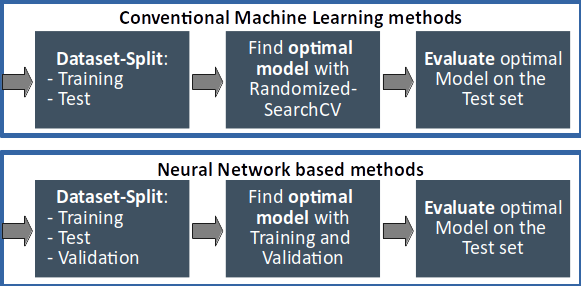
\includegraphics[width=0.7\linewidth]{figures/classifier_pipeline.png}
	\caption{Classifier pipeline}
	\label{fig:classifier_pipeline}
\end{figure}

For the conventional machine learning methods the dataset is split into training (0.8) and test set (0.2). In order to find the optimal model \textit{Randomized\-SearchCV} is executed on the defined hyperparameter search space. The hyperparameter search space was chosen based on the classifiers doc\-u\-men\-ta\-tion, papers and by an empirical examination. For the Decision Tree we followed \cite{mantovani2019empirical} and for the Random Dorest \cite{probstHyperparametersTuningStrategies2019}. For SVM we used the sklearn C-Support Vector Classification implementation and concentrated the randomized search on the kernel (linear, poly, rbf or sigmoid) as this has the biggest impact on performance. Tuning the kernel already used up quite some computational time, so we did not look into further parameters. In future work one could have a closer look at parameters such as the regularization parameter C or some kernel specific coefficients. To train the Logistic Regression model, hyperparameters were set according to the recommendations from sklearns documentation page. To try out different solver algorithms, the L2-norm penalty for regularization was chosen. As the number of samples surpass the number of features the normal primal formulation of the regression problem was used. The search space for solver algorithms was restricted to \textit{lbfgs}, \textit{sag} and \textit{saga} as others did not make sense in the training circumstances. Also different regularization strength was tested with parameter C between 0.8 and 1.2 with step width 0.1. Finally the model is evaluated on the test set.

For neural network based approaches the dataset is again split into training (0.8) and test set (0.2). Then the training set is further split up into training (0.8) and validation (0.2). In the next step the optimal model is found by using the training and the validation set. The final step is equal to the final step in conventional machine learning, were the model is evaluated.

To enable a performant execution Pythons multiprocessing library is used to parallelize the execution.

\subsection{Evaluation}
\label{ch:approachE}

For evaluating the classifiers standard metrics such as accuracy, precision, recall and F1 score are used.

The accuracy specifies how many data instances are correctly classified. Only looking at the accuracy, is not that informative, because generally a lot of instances are correctly classified as non hate speech, which leads to a high accuracy. That is why also precision and recall are observed. Precision specifies how many of the predicted hate speech instances are really hate speech. A low precision means that many instances are classified as hate speech, although they are not. So looking at the precision enables us to detect if the trained model could be used as a censoring system and undermine the freedom of speech. The recall specifies how many hate speech instances are correctly classified by the model. A low recall means that there are many false negatives (a lot of hate speech instances are not detected). For taking into account precision and recall one can look at the F1 score.

